% Created 2016-09-28 Wed 22:40
\documentclass[dvipdfmx,presentation]{beamer}
\usepackage{pxjahyper}
\usepackage{beamerthemeshadow}
\usepackage[utf8x]{inputenc}
\usepackage[T1]{fontenc}
\usepackage{txfonts}
\usepackage{textcomp}
\usepackage[french, english, japanese]{babel}
\usetheme{Antibes}
\usefonttheme[onlymath]{serif}
\def\bf{\mathbf}
\usetheme{default}
\author{Makoto Otsuka}
\date{2016-08-26 Fri}
\title{Chapter 20: Deep Generative Models\\
}
\subtitle{Deep Learning Book by I. Goodfellow, Y. Bengio and A. Courville \\
OIST Deep Learning Reading Group}
\hypersetup{
 pdfauthor={Makoto Otsuka},
 pdftitle={Chapter 20: Deep Generative Models\\
},
 pdfkeywords={},
 pdfsubject={},
 pdfcreator={Emacs 24.5.1 (Org mode 8.3.4)}, 
 pdflang={English}}
\begin{document}

\maketitle
\begin{frame}{Outline}
\tableofcontents
\end{frame}


\section{20.6 Convolutional Boltzmann Machines}
\label{sec:orgheadline3}
\begin{frame}[label={sec:orgheadline1}]{20.6 Convolutional Boltzmann Machines}
\begin{itemize}
\item High dimensional inputs (e.g., images) requires computational, memory, and statistical resources
\item Approach: Use convolution
\begin{itemize}
\item Works well also with RBM (Desjardins and Bengio, 2008)
\item Difficult to generalize \alert{\alert{pooling operation}} in energy-based model
\begin{itemize}
\item \(2^{9} = 512\) energy function evaluations per \(3\times3\) pooling units
\end{itemize}
\end{itemize}
\end{itemize}
\begin{block}{Probabilistic max pooling (Lee et al, 2009)}
\begin{itemize}
\item At most one unit may be active at a time
\begin{itemize}
\item \(n+1\) possible states
\item \(+1\) for the states with all units off (E = 0)
\end{itemize}
\item No overlapoing pooling regions :(
\end{itemize}
\end{block}
\end{frame}


\begin{frame}[label={sec:orgheadline2}]{20.6 Convolutional Boltzmann Machines}
\begin{block}{Convolutional DBM with probabilistic max pooling (Lee et al, 2009)}
\begin{itemize}
\item Pros
\begin{itemize}
\item Possible to fill in the missing portions of its input
\end{itemize}
\item Cons
\begin{itemize}
\item Challenging to make it work in practice
\item CNNs with supervised training objective usually perfoms better
\item Cannot change the size of pooling region to accept images in different sizes
\begin{itemize}
\item Partition function changes as the size of the input changes
\item Variable sized inputs can be accepted if output feature maps can be scaled automatically
\end{itemize}
\item Difficult to handle image boundary
\end{itemize}
\end{itemize}
\end{block}
\end{frame}

\section{20.7 Boltzmann Machine for Structured or Sequential Outputs}
\label{sec:orgheadline5}
\begin{frame}[label={sec:orgheadline4}]{20.7 Boltzmann Machine for Structured or Sequential Outputs}
\begin{itemize}
\item Tools for modeling structured ouput can be used for modeling sequences
\item Conditional RBM (Taylor et al., 2007)
\item Conditional RBM + spectral hashing (Mnih et al., 2011)
\item Factored conditional RBM for modeling motion style (Taylor and Hinton, 2009)
\item RTRBM (Sutskever, Hinton, Taylor, 2009)
\item RNN-RBM for learning musical notes (Boulanger-Lewandowski et al., 2012)
\end{itemize}
\end{frame}

\section{20.8 Other Boltzmann Machines}
\label{sec:orgheadline7}
\begin{frame}[label={sec:orgheadline6}]{20.8 Other Boltzmann Machines}
\begin{itemize}
\item Discriminative RBMs (Larochelle and Bengio, 2008)
\begin{itemize}
\item maximize \(\log p(y | \mathbf{v})\)
\end{itemize}
\item Higher-order BMs
\begin{itemize}
\item Higher-order BMs (Sejnowski, 1987)
\item Mixture of RBMs (Nair and Hinton, 2009)
\item Two groups of hidden units (Luo et al., 2011)
\item Point-wise gated BMs (PGBMs) (Sohn et al. 2013)
\end{itemize}
\end{itemize}
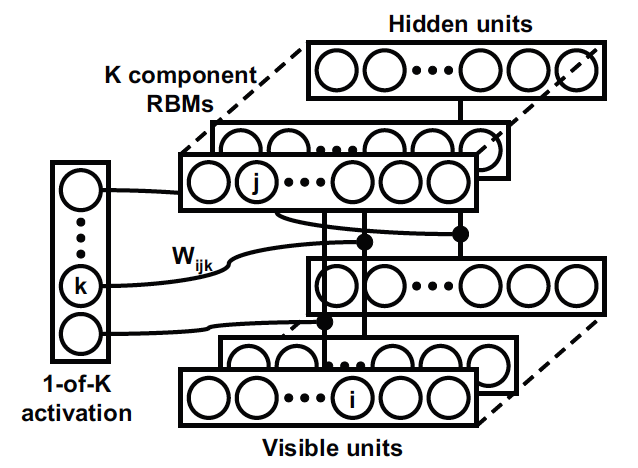
\includegraphics[width=0.30\textwidth]{./figure/nair2009fig1b.png}
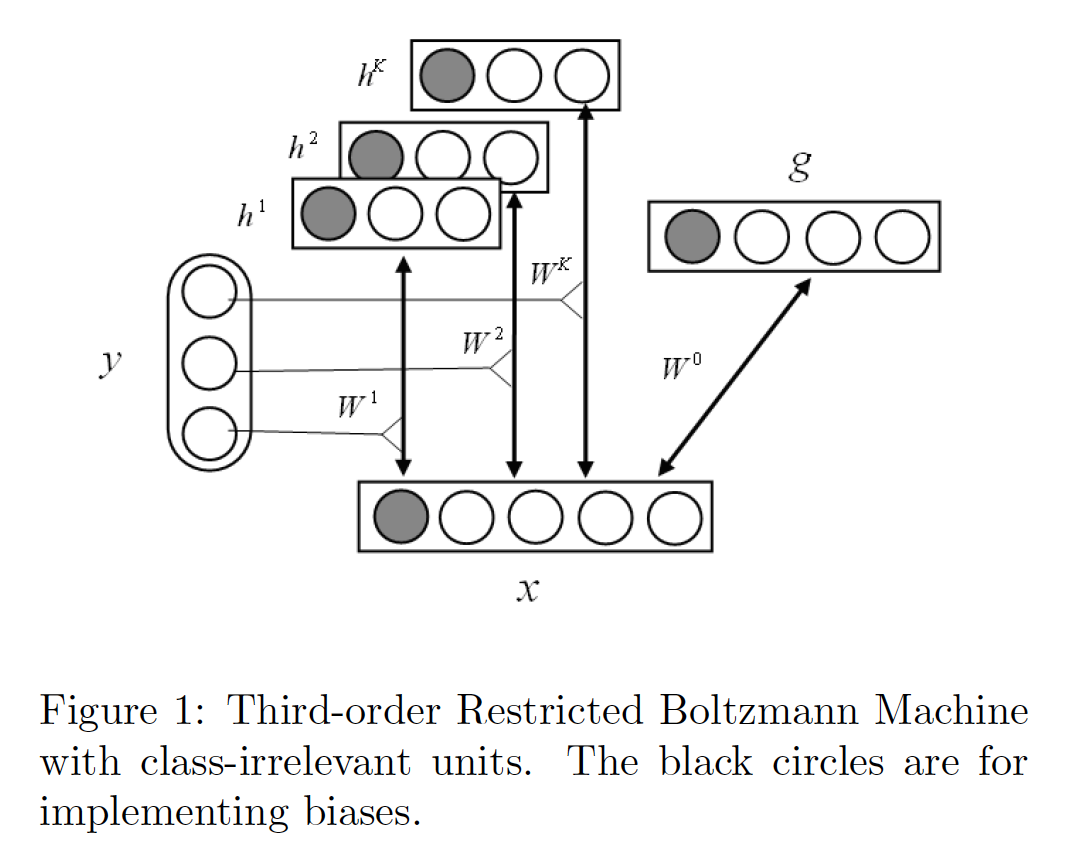
\includegraphics[width=0.30\textwidth]{./figure/luo2011fig1.png}
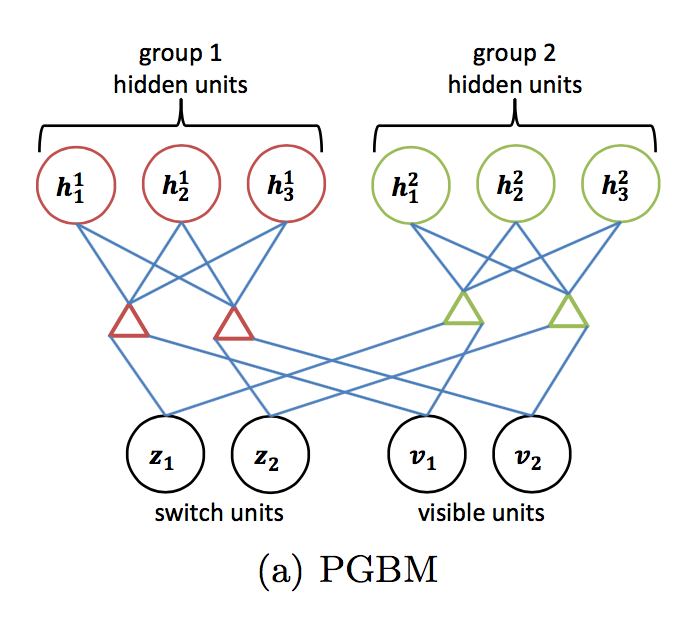
\includegraphics[width=0.30\textwidth]{./figure/sohn2013fig1a.png}
\end{frame}

\section{20.9 Back-Propagation through Random Operations}
\label{sec:orgheadline11}
\begin{frame}[label={sec:orgheadline8}]{20.9 Back-Propagation through Random Operations}
\begin{itemize}
\item \(\bf{x}\): input variable
\item \(\bf{z}\): simple distribution (e.g., uniform, Gaussian)
\item \(f(\bf{x}, \bf{z})\) appears stochastic
\item If \(f\) is continuous and differentiable, we can apply BP as usual
\end{itemize}
\end{frame}

\begin{frame}[label={sec:orgheadline9}]{Example: Drawing samples from a Gaussian distribution}
\begin{itemize}
\item It seems counter intuitive to take a derivative of the sampling process \(y\) with respect to \(\mu\) or \(\sigma\)
\end{itemize}

\centering
\(y \sim \mathcal{N}(\mu, \sigma^{2})\)
\begin{itemize}
\item But it make sense if we rewrite this sampling process as follows:
\end{itemize}
\centering
\(y = \mu + \sigma z$, $\quad z \sim \mathcal{N}(0, 1)\)
\begin{itemize}
\item Note that \(z\) does not depend on \(\mu\) nor \(\sigma\)
\end{itemize}
\centering
\(\mu = g_{1}(\bf{x}; \theta_{1}), \quad \sigma = g_{2}(\bf{x}; \theta_{2})\)
\end{frame}

\begin{frame}[label={sec:orgheadline10}]{Reparametrization trick}
\begin{itemize}
\item Reparameterization trick (stochastic back-propagation, perturbation analysis)
\item \(\bf{\omega}\): a variable containing both parameters \(\theta\), and if applicable, the inputs \(\bf{x}\)
\item We can rewrite
\end{itemize}
\centering
\(y \sim p(y | \omega)\)

as

\(y = f(z; \omega) = \mu_{\theta_{1}} + \sigma_{\theta_{2}} z\)
\begin{itemize}
\item \(\omega\) is not the function of \(\bf{z}\)
\item \(\bf{z}\) is not the function of \(\omega\)
\end{itemize}
\end{frame}
\section{20.10 Directed Generative Nets}
\label{sec:orgheadline43}
\begin{frame}[label={sec:orgheadline12}]{20.10 Directed Generative Nets}
\begin{itemize}
\item Since 2013, directed generative nets became popular
\item 20.10.1 Sigmoid Belief Nets
\item 20.10.2 Differentiable Generator Nets
\item 20.10.3 Variational Autoencoders (VAEs)
\item 20.10.4 Generative Adversarial Networks (GANs)
\item 20.10.5 Generative Moment Matching Networks
\item 20.10.6 Convolutional Generative Networks
\item 20.10.7 Auto-Regressive Networks
\item 20.10.8 Linear Auto-Regressive Networks
\item 20.10.9 Neural Auto-Regressive Networks
\item 20.10.10 Neural autoregressive density estimator (NADE)
\end{itemize}
\end{frame}
\begin{frame}[label={sec:orgheadline13}]{20.10.1 Sigmoid Belief Nets}
\begin{itemize}
\item Proposed by Neal (1990)
\item Universal approximator of binary visible units (Sutskever and Hinton, 2008)
\item Inferece is hard
\begin{itemize}
\item Mean field inference is intractable
\item Approximate lowerbound (Saul et al., 1996) is only applicable for small networks
\item SBNs combined with an inference net need to rely on unreliable BP through discrete sampling processes
\end{itemize}
\item Recent approaches enable fast training
\begin{itemize}
\item Importance sampling + reweighted wake-sleep (Bornschein and Bengio, 2015)
\item Bidirectional Helmnoltz machines (Bornschein et al, 2015)
\end{itemize}
\end{itemize}
\end{frame}

\begin{frame}[label={sec:orgheadline14}]{20.10.2 Differentiable Generator Nets}
\begin{itemize}
\item The model transforms samples of latent varialbes \(\bf{z}\) to 
\begin{itemize}
\item samples \(\bf{x}\) directly (Approach 1) or
\item distributions over samples \(\bf{x}\) (Approach 2)
\end{itemize}
using differentiable function \(g(\bf{z}; \theta^{(g)})\) (usually NN)
\item Parameterized computational procedures for generating samples
\item Examples
\begin{itemize}
\item Variational autoencoders (VAE)
\begin{itemize}
\item generator net + inference net
\end{itemize}
\item Generative adversarial networks (GAN)
\begin{itemize}
\item generator net + discriminator net
\end{itemize}
\item Generative moment matching networks
\end{itemize}
\end{itemize}
\end{frame}

\begin{frame}[label={sec:orgheadline15}]{Approach 1: Direct Sampling (1/2)}
\begin{itemize}
\item Generating samples from a multivariate Gaussian distribution
\begin{itemize}
\item \(\bf{z} \sim \mathcal{N}(\bf{0}, I)\)
\item \(g(\bf{z}; \theta^{(g)})\) is given by
\end{itemize}
\end{itemize}
\begin{align*}
\bf{x} &= g(\bf{z}; \theta^{(g)}) = \bf{\mu} + \bf{L} \bf{z} \tag{20.71}\\
\Sigma &= \bf{L} \bf{L}^{\top} \quad \cdots \text{Cholesky decomposition}
\end{align*}

\begin{itemize}
\item Inverse transform sampling (Devroye, 2013)
\begin{itemize}
\item \(z \sim U(0, 1)\)
\item \(g(z)\) is given by the inverse of the cdf \(F(x) = \int_{-\infty}^{x} p(v) dv\)
\end{itemize}

\item \(g()\) is transforming the distribution over \(\bf{z}\) into the desired distribution over \(\bf{x}\)
\end{itemize}
\end{frame}

\begin{frame}[label={sec:orgheadline16}]{Approach 1: Direct Sampling (2/2)}
\begin{itemize}
\item For invertible, differentiable, continuous \(g\),
\end{itemize}

\begin{align*}
p_{x}(\bf{x}) d \bf{x} &= p_{z}(\bf{z}) d \bf{z} \\
p_{x}(g(\bf{z})) \left| \det (\frac{\partial g}{\partial \bf{z}}) \right| &= p_{z}(\bf{z}) \tag{20.72} \\
p_{x}(\bf{x}) &= \frac{p_{z}(g^{-1}(\bf{x}))}{\left| \det (\frac{\partial g}{\partial \bf{z}}) \right|} \tag{20.73}
\end{align*}

where \(\bf{x} = g(\bf{z})\)

\begin{itemize}
\item Usually difficult to evaluate \(\log p(\bf{x})\) directly
\item Often use indirect means of learning \(g(\cdot)\)
\end{itemize}
\end{frame}

\begin{frame}[label={sec:orgheadline17}]{Approach 2: Defining conditional distribution}
\begin{itemize}
\item Defining conditional distribution
\end{itemize}

\begin{align*}
p(x_{i} = 1 | \bf{z}) &= g(\bf{z})_{i} \tag{20.74} \\
\end{align*}

\begin{itemize}
\item Marginalizing it out to define \(p_{g}(\bf{x})\)
\end{itemize}

\begin{align*}
p(\bf{x}) &= \mathbf{E}_{\bf{z}} p(\bf{x} | \bf{z}) \tag{20.75}
\end{align*}
\end{frame}

\begin{frame}[label={sec:orgheadline18}]{Direct sampling v.s. defining conditional distribution}
\begin{itemize}
\item Approach 1: Emitting samples directly from \(p_{g}(\bf{x})\)
\begin{itemize}
\item Pros
\begin{itemize}
\item No longer forced to use carefully-designed conditional distributions
\end{itemize}
\item Cons
\begin{itemize}
\item Capable of generating only continuous data
\end{itemize}
\end{itemize}
\item Approach 2: Emitting parameters of \(p_{g}(\bf{x})\)
\begin{itemize}
\item Pros
\begin{itemize}
\item Capable of generating discrete data as well as continuous data
\end{itemize}
\item Cons
\begin{itemize}
\item Need to use carefully-designed conditional distributions
\end{itemize}
\end{itemize}
\end{itemize}
\end{frame}

\begin{frame}[label={sec:orgheadline19}]{Properties of Differentiable Generator Nets}
\begin{itemize}
\item Diffrentiable generator nets were motivated by the success of BP applied to SL
\item But unsupervised generative modeling is more difficult than SL
\item Differentiable generator nets need to solve two objectives
\begin{itemize}
\item How to arrange \(\bf{z}\) space in a useful way
\item How to map from \(\bf{z}\) to \(\bf{x}\)
\end{itemize}
\item Chair generation experiment (Dosovitskiy et al., 2015)
\begin{itemize}
\item Mapping between \(\bf{z}\) and \(\bf{x}\) is given beforehand (mapping is deterministic)
\item Result implies DGNs have sufficient model capacity and it is optimizable
\item But, don't know what happends when mapping between \(\bf{z}\) and \(\bf{x}\) is non-deterministic
\end{itemize}
\end{itemize}
\end{frame}

\begin{frame}[label={sec:orgheadline20}]{20.10.3 Variational Autoencoders (VAEs)}
\begin{itemize}
\item Proposed by Kingma (2013) and Rezende et al. (2014)
\item Directed model that use learned approximate inference
\item Can be trained purely with gradient-based methods
\item Great blog posts about VAEs: \href{http://blog.fastforwardlabs.com/post/148842796218/introducing-variational-autoencoders-in-prose-and}{(link 1}, \href{http://blog.fastforwardlabs.com/post/149329060653/under-the-hood-of-the-variational-autoencoder-in}{link 2})
\end{itemize}
\begin{block}{Building blocks of VAE}
\begin{itemize}
\item \(p_{\mathrm{model}}(\bf{z})\quad\) Code distribution (prior)
\item \(g(\bf{z}; \theta^{(g)})\quad\) Differentiable generator net (decoder)
\item \(p_{\mathrm{model}}(\bf{x} | \bf{z}) = p_{\mathrm{model}}(\bf{x}; g(\bf{z}; \theta^{(g)}))\quad\) Generative model
\item \(f(\bf{x}; \theta^{(f)})\quad\) Approximate inference net (encoder)
\item \(q(\bf{z} | \bf{x}) = q(\bf{z}; f(\bf{x}; \theta^{(f)}))\quad\) Recognition model
\end{itemize}
\end{block}
\end{frame}





\begin{frame}[label={sec:orgheadline21}]{Training VAEs}
\begin{itemize}
\item Instead of directly maximizing log likelihood
\end{itemize}
\begin{align*}
\log p_{\mathrm{model}} (\bf{x}) &= \mathcal{L}(q) + D_{\mathrm{KL}}(q(\bf{z} | \bf{x}) || p_{\mathrm{model}}(\bf{z} | \bf{x}))
\end{align*}

\begin{itemize}
\item Train VAE by maximizing variational lower bound \(\mathcal{L}(q)\)
\end{itemize}
\begin{align*}
\mathcal{L}(q) 
&= 
\bf{E}_{\bf{z} \sim q(\bf{z} | \bf{x})} \log p_{\mathrm{model}}(\bf{z}, \bf{x}) 
+ \mathcal{H}(q(\bf{z} | \bf{x})) \tag{20.76}\\
&= \bf{E}_{\bf{z} \sim q(\bf{z} | \bf{x})} \log p_{\mathrm{model}}(\bf{x} | \bf{z})
+ \bf{E}_{\bf{z} \sim q(\bf{z} | \bf{x})} \log p_{\mathrm{model}}(\bf{z})
- \bf{E}_{\bf{z} \sim q(\bf{z} | \bf{x})} \log q(\bf{z} | \bf{x}) \\
&= 
\bf{E}_{\bf{z} \sim q(\bf{z} | \bf{x})} \log p_{\mathrm{model}}(\bf{x} | \bf{z})
- D_{\mathrm{KL}}( q(\bf{z} | \bf{x}) || p_{\mathrm{model}}(\bf{z})) \tag{20.77}\\
&\le \log p_{\mathrm{model}} (\bf{x}) \tag{20.78}
\end{align*}

\begin{itemize}
\item Interpretation
\begin{itemize}
\item \(\mathcal{H}(q(\bf{z} | \bf{x}))\) encourages higher variance
\item \(D_{\mathrm{KL}}( q(\bf{z} | \bf{x}) || p_{\mathrm{model}}(\bf{z}))\) encourages smaller distance between approximate posterior and prior
\item \(\bf{E}_{\bf{z} \sim q(\bf{z} | \bf{x})} \log p_{\mathrm{model}}(\bf{x} | \bf{z})\) encourages lower reconstruction error
\end{itemize}
\end{itemize}
\end{frame}

\begin{frame}[label={sec:orgheadline22}]{Traditional approach to variational inference and learning}
\begin{itemize}
\item Infer \(q(\cdot)\) via optimization algorithm (e.g., iterated fixed point equations)
\item Iterative scheme is slow
\item Often require the ability to compute \(\bf{E}_{\bf{z} \sim q} \log p_{\mathrm{model}}(\bf{z}, \bf{x})\) in closed form
\end{itemize}
\end{frame}

\begin{frame}[label={sec:orgheadline23}]{Main idea behind VAE}
\begin{itemize}
\item Train a parameteric encoder \(f(\bf{x}; \theta^{(f)})\) for \(q(\bf{z} | \bf{x}) = q(\bf{z}; f(\bf{x}; \theta^{(f)}))\)
\item If \(\bf{z}\) is continuous, we can use BP
\item All the expectation in \(\mathcal{L}\) may be approximated by MC sampling
\end{itemize}
\end{frame}

\begin{frame}[label={sec:orgheadline24}]{Shortcomings of VAE}
\begin{enumerate}
\item Generated images are blurry probably due to
\begin{itemize}
\item ML estimate
\begin{itemize}
\item Minimizing \(D_{\mathrm{KL}}(p || q)\) instead of \(D_{\mathrm{KL}}(q || p)\)
\item Tendency to ignore small changes in images (Theis et al., 2015; Huszar 2015)
\end{itemize}
\item Use of Gaussian model \(p_{\mathrm{model}}(\bf{x}; g(\bf{z}))\)
\end{itemize}
\end{enumerate}
\centering
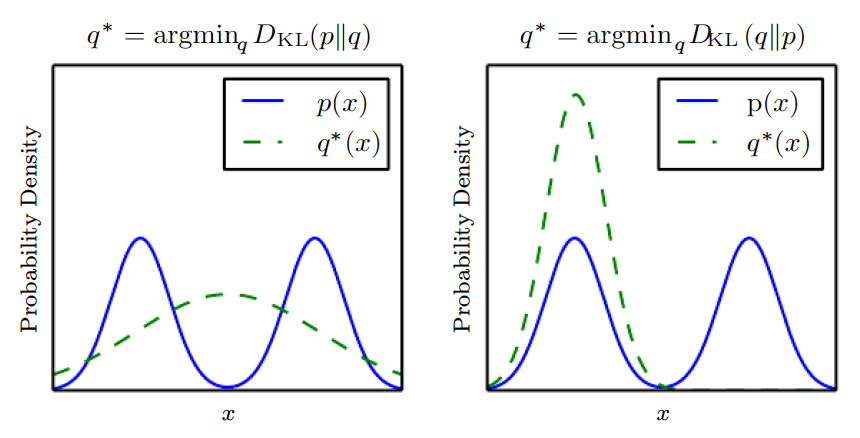
\includegraphics[width=0.60\textwidth]{./figure/dlbook_fig3_6.png}
\begin{enumerate}
\item Tend to use only small subset of \(\bf{z}\)
\end{enumerate}
\end{frame}

\begin{frame}[label={sec:orgheadline25}]{Extension of VAE (1/2)}
\begin{itemize}
\item VAE is much easier to extend than Boltzmann machines
\item Deep recurrent attention writer (DRAW) model (Gregor et al., 2015)
\begin{itemize}
\item Recurrent encoder + recurrent decoder + attention
\end{itemize}
\item Variational RNNs (Chung et al, 2015b)
\begin{itemize}
\item Recurrent encoder and decoder
\item Unlike traditional RNN, it also has variability in latent space
\end{itemize}
\item Importance weighted autoencoder or IWAE (Burda et al., 2015) objective
\begin{itemize}
\item Equivalent to the traditional lower bound when \(k=1\)
\item Tighter bound for \(\log p_{\mathrm{model}}(\bf{x})\) when \(k\) increases
\end{itemize}
\end{itemize}
\begin{align*}
\mathcal{L}_{k}(\bf{x}, q) = \bf{E}_{\bf{z}^{(1)}, \ldots, \bf{z}^{(k)} \sim q(\bf{z} | \bf{x})}
\left[
\log \frac{1}{k} \sum_{i=1}^{k} \frac{p_{\mathrm{model}(\bf{x}, \bf{z}^{(i)})}}{q(\bf{z}^{(i)} | \bf{x})}
\right]
\end{align*}
\end{frame}

\begin{frame}[label={sec:orgheadline26}]{Extension of VAE (2/2)}
\begin{itemize}
\item Some interesting connections to the multi-prediction DBM (MP-DBM) in Fig. 20.5 and other approaches that involve back-propagation through the approximate inference graph (Goodfellow et al., 2013b; Stoyanov et al., 2011; Brakel et al., 2013).
\item VAE is defined for arbitrary computational graphs
\begin{itemize}
\item No need to restrict the choice of models to those with tractable mean field fixed point equations
\end{itemize}
\item One disadvantage of the variational autoencoder is that it learns an inference network for only one problem, inferring \(\bf{z}\) given \(\bf{x}\).
\end{itemize}
\end{frame}

\begin{frame}[label={sec:orgheadline27}]{Manifold learning with VAE}
\centering
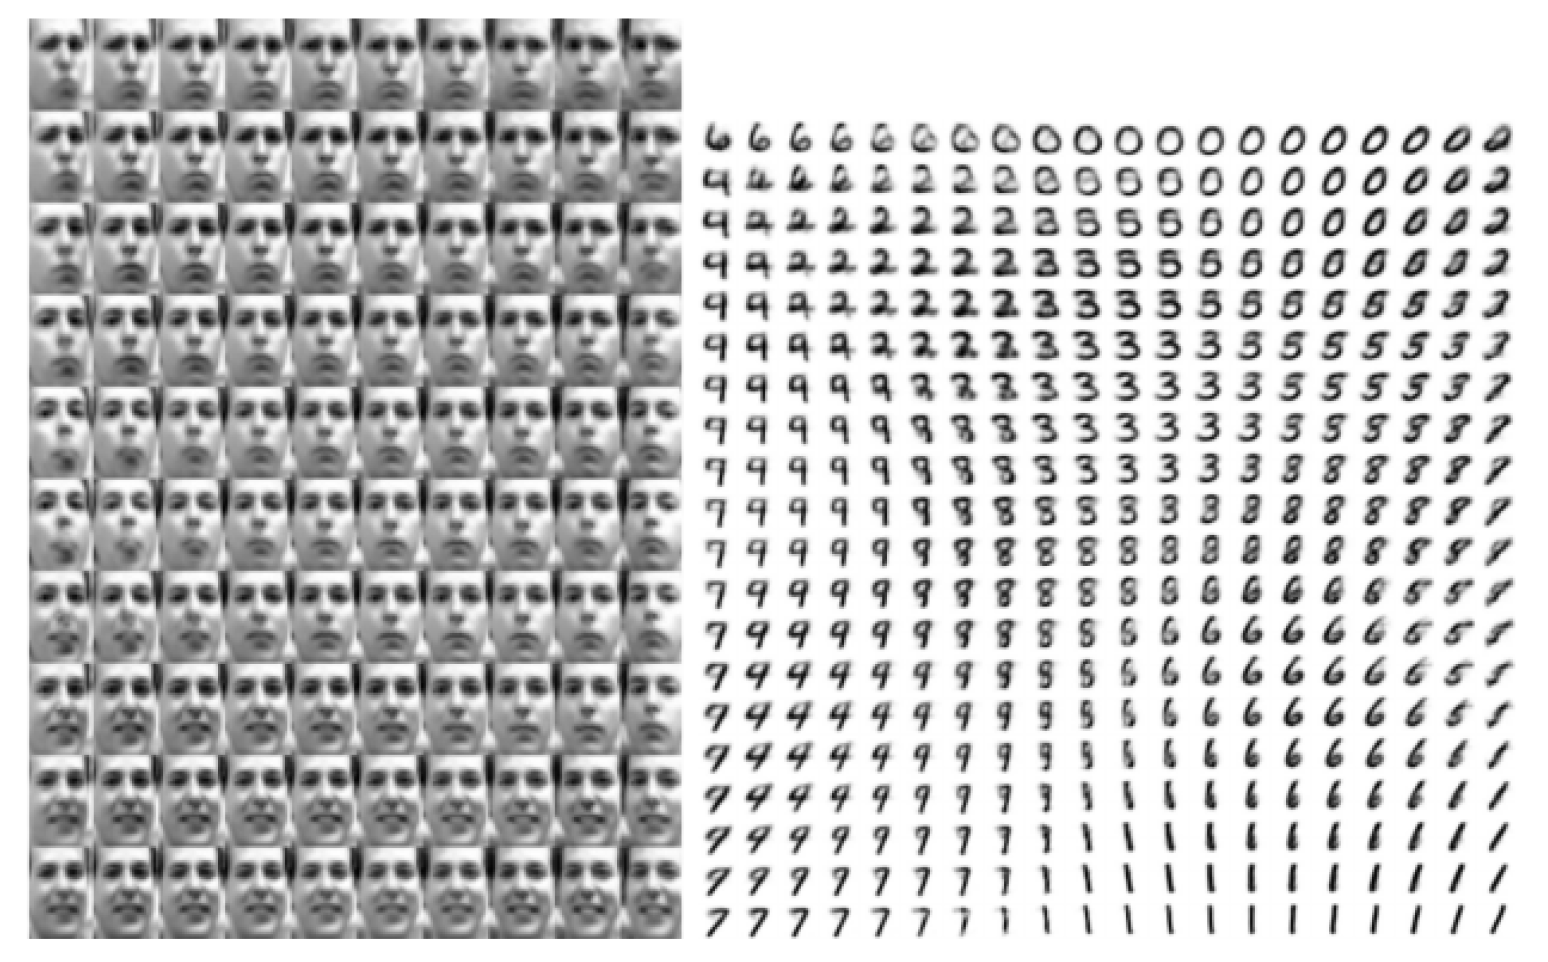
\includegraphics[width=0.90\textwidth]{./figure/dlbook_fig20_6.png}
\end{frame}

\begin{frame}[label={sec:orgheadline28}]{20.10.4 Generative Adversarial Networks (GANs)}
\begin{itemize}
\item Proposed by Goodfellow et al. (2014c)
\item Example of differentiable generator networks
\item Generator net: \(g(\bf{z}; \theta^{(g)})\)
\begin{itemize}
\item Directly produces samples: \(\bf{x} = g(\bf{z}; \theta^{(g)})\)
\item Payoff is \(- v(\theta^{(g)}, \theta^{(d)})\)
\item Attempts to fool the classifier into believing its samples are real
\end{itemize}
\item Discriminator net: \(d(\bf{x}; \theta^{(d)})\) (probability of \(\bf{x}\) being real)
\begin{itemize}
\item Payoff is \(v(\theta^{(g)}, \theta^{(d)})\)
\item Attempts to learn to correctly classify samples as real or fake
\end{itemize}
\end{itemize}
\begin{align*}
g* &= \arg \min_{g} \max_{d} v(g, d) \\
v(\theta^{(g)}, \theta^{(d)}) &= \bf{E}_{\bf{x} \sim p_{\mathrm{data}}} \log d(\bf{x})
+ \bf{E}_{\bf{x} \sim p_{\mathrm{model}}} \log (1 - d(\bf{x}))
\end{align*}
\end{frame}

\begin{frame}[label={sec:orgheadline29}]{Difficulties in GANs}
\begin{itemize}
\item Learning is difficult in GAN
\begin{itemize}
\item E.g.) \(v(a, b) = a b\)
\item Note that the equilibria for a minimax game are not local minima of \(v\)
\item Instead, they are points that are simultaneously minima for both players' costs.
\item This means that they are saddle points of \(v\) that are local minima with respect to the first player's parameters and local maxima with respect to the second player's parameters.
\end{itemize}
\item Alternative formulation of payoffs (Goodfellow et al., 2014c)
\end{itemize}
\end{frame}
\begin{frame}[label={sec:orgheadline30}]{Deep convolutional GAN (DCGAN)}
\begin{itemize}
\item Proposed by Radford et al. (2015)
\end{itemize}
\begin{columns}
\begin{column}{0.50\columnwidth}
\centering
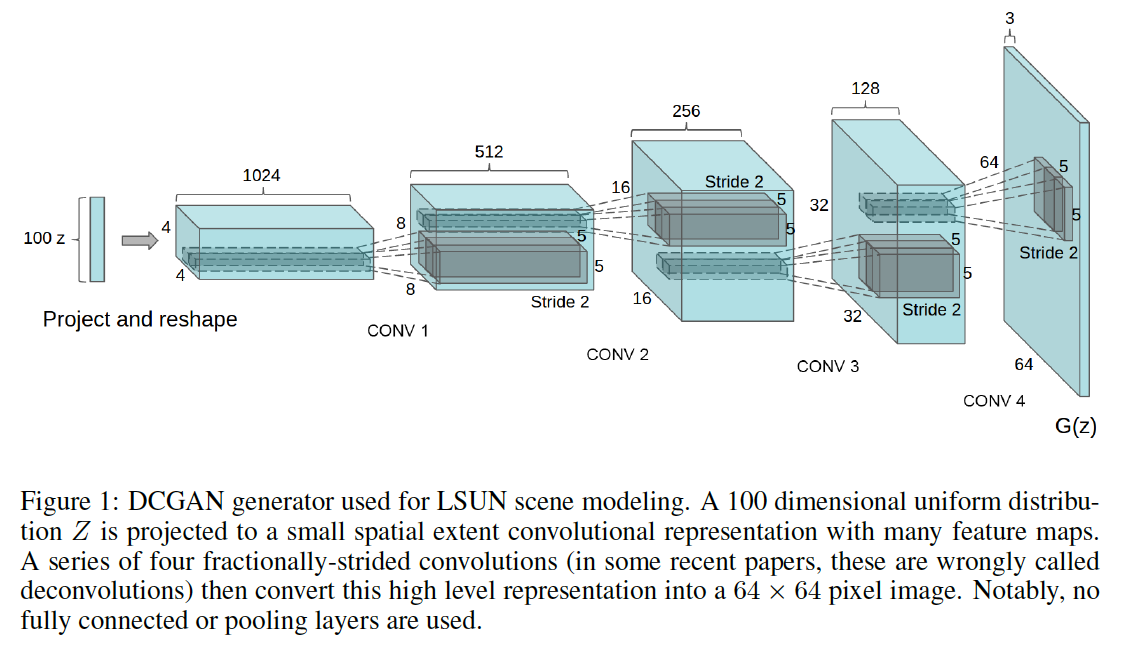
\includegraphics[width=\textwidth]{./figure/radford2015fig1.png}
\end{column}
\begin{column}{0.50\columnwidth}
\centering
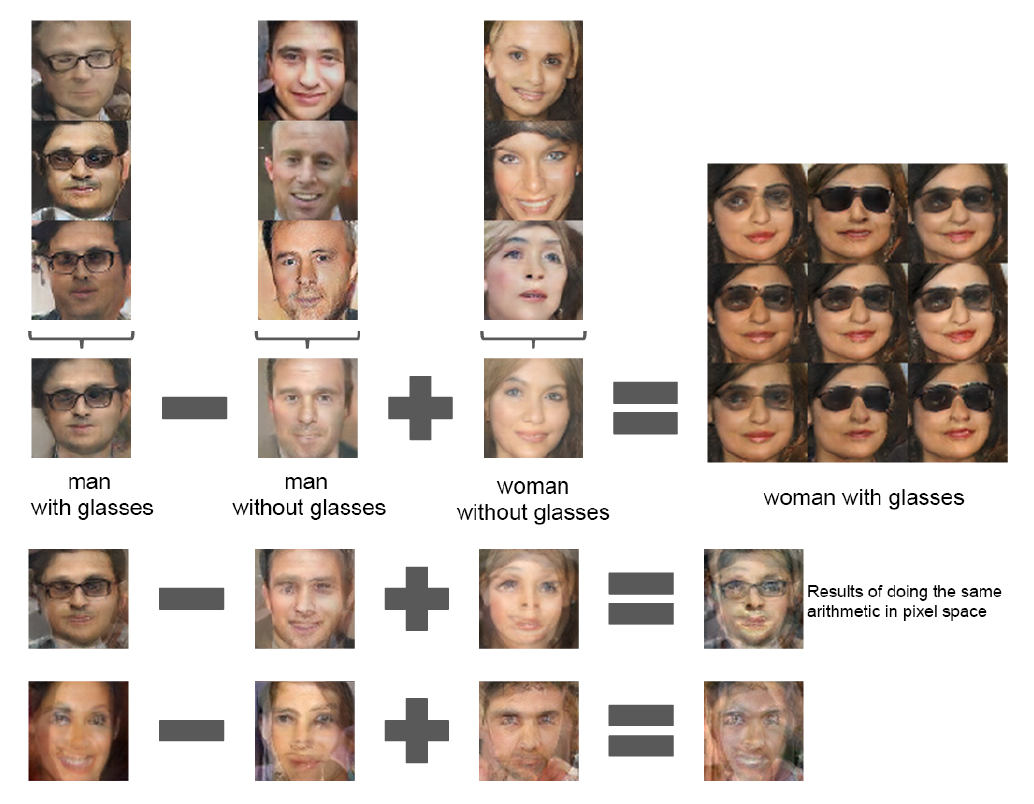
\includegraphics[width=\textwidth]{./figure/radford2015fig7.png}
\end{column}
\end{columns}
\end{frame}

\begin{frame}[label={sec:orgheadline31}]{Conditional GANs and LAPGAN}
\begin{itemize}
\item Conditional GANs (Mirza and Osindero, 2014)
\begin{itemize}
\item Learn to sample from \(p(\bf{x} | \bf{y})\) rather than \(p(\bf{x})\)
\end{itemize}
\item LAPGAN (Denton et al. 2015) uses series of conditional GANs with Laplacian pyramid
\end{itemize}
\centering
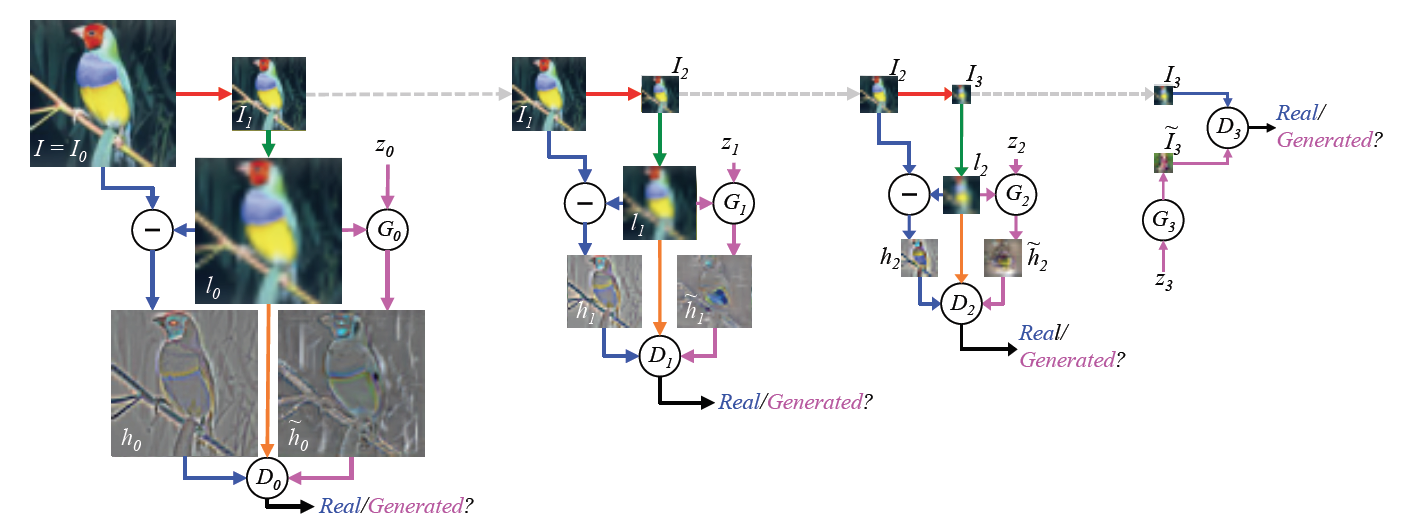
\includegraphics[width=\textwidth]{./figure/denton2015fig2.png}
\end{frame}

\begin{frame}[label={sec:orgheadline32}]{Generated Images: DCGAN and LAPGAN}
\centering
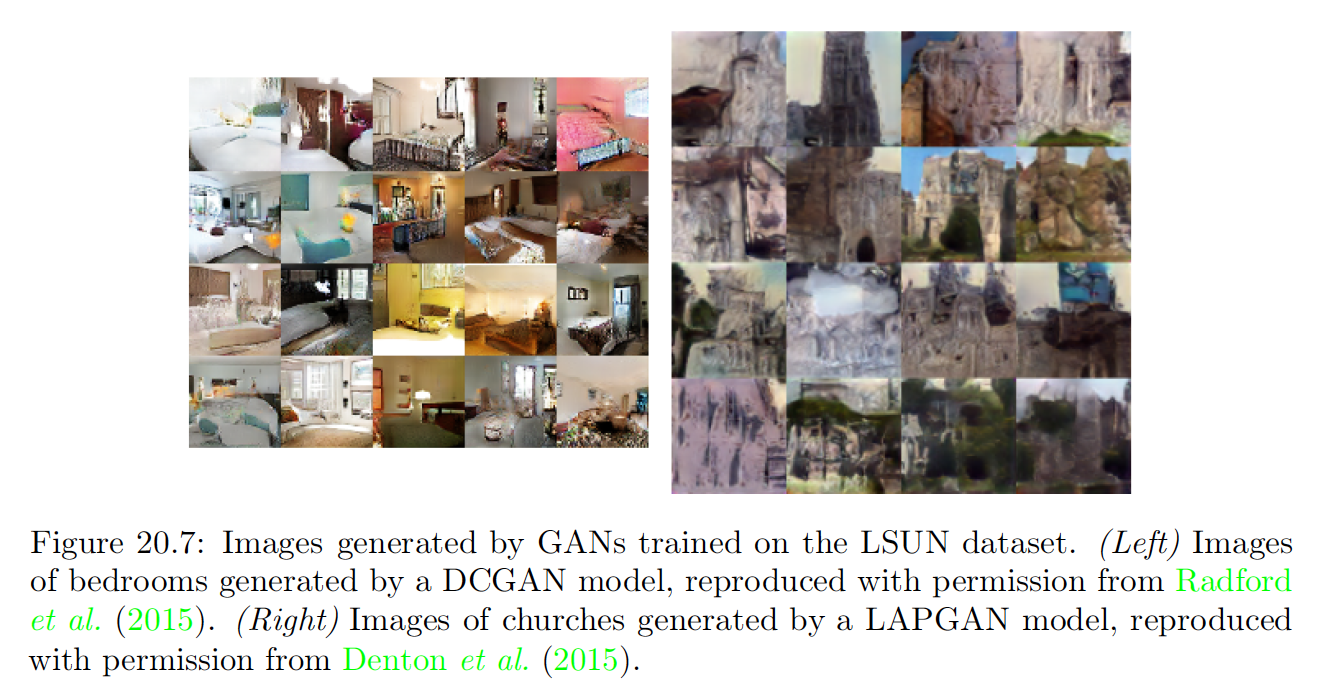
\includegraphics[width=1.0\textwidth]{./figure/dlbook_fig20_7.png}
\end{frame}

\begin{frame}[label={sec:orgheadline33}]{Properties of GAN}
\begin{itemize}
\item It can fit distribution that assign zero probability to the training points.
\item Somehow tracing out manifold that is spanned by training data
\item Add Gaussian noise to all of the generated values to ensure non-zero probabilities to all points
\item Dropout seems to be important in the discriminator network
\begin{itemize}
\item In particular, units should be stochastically dropped while computing the gradient for the generator network to follow.
\end{itemize}
\end{itemize}
\end{frame}

\begin{frame}[label={sec:orgheadline34}]{Models similar to GAN}
\begin{itemize}
\item GAN is designed for differentiable generator net.
\item Similar principles can be used to train other kind of models
\item \alert{\alert{Self-supervised boosting}} can be used to train RBM generator to fool a logistic regression discriminator (Welling et al., 2002)
\end{itemize}
\end{frame}

\begin{frame}[label={sec:orgheadline35}]{20.10.5 Generative Moment Matching Networks}
\begin{itemize}
\item Proposed by Li et al., 2015; Dziugaite et al., 2015
\item Example of differentiable generator networks
\item Unlike VAEs and GANs, no need to pair with other network
\item Trained with \alert{\alert{moment matching}}
\end{itemize}
\begin{align*}
\bf{E}_{\bf{x}} \prod_{i} x_{i}^{n_{i}} \tag{20.82}\\
\bf{n} = [n_{1}, \ldots, n_{d}]^{\top}
\end{align*}

\begin{itemize}
\item Matching all moment for all dimensions is infeasible
\item Instead, minimize the maximum mean discrepancy, MMD (Scholkopf and Smola, 2002; Gretton et al., 2012)
\begin{itemize}
\item Measures the error in the first moments in an infinite-dimensional space implicitly defined by kernel
\item MMD cost is 0 if and only if the two distributions being compared are equal
\end{itemize}
\end{itemize}
\end{frame}

\begin{frame}[label={sec:orgheadline36}]{Generative Moment Matching Networks}
\begin{itemize}
\item Samples from GMMN is not visually pleasing
\item Visual can be improved if generator is combined with an autoencoder
\item Need large batch size to obtain reliable estimate of the moment
\end{itemize}
\end{frame}

\begin{frame}[label={sec:orgheadline37}]{20.10.6 Convolutional Generative Networks}
\begin{itemize}
\item When generating images, it is useful to include convoluitonal structure (Goodfellow et al., 2014c; Dosovitskiy et al., 2015)
\item Pooling function is not invertible
\item "Un-pooling" (Dosovitskiy et al., 2015) 
\begin{itemize}
\item Inverse of max-pooling
\item Upper-left corner takes maximum value and other cells are set to 0
\item Samples generated by the model are visually pleasing
\end{itemize}
\end{itemize}

\centering
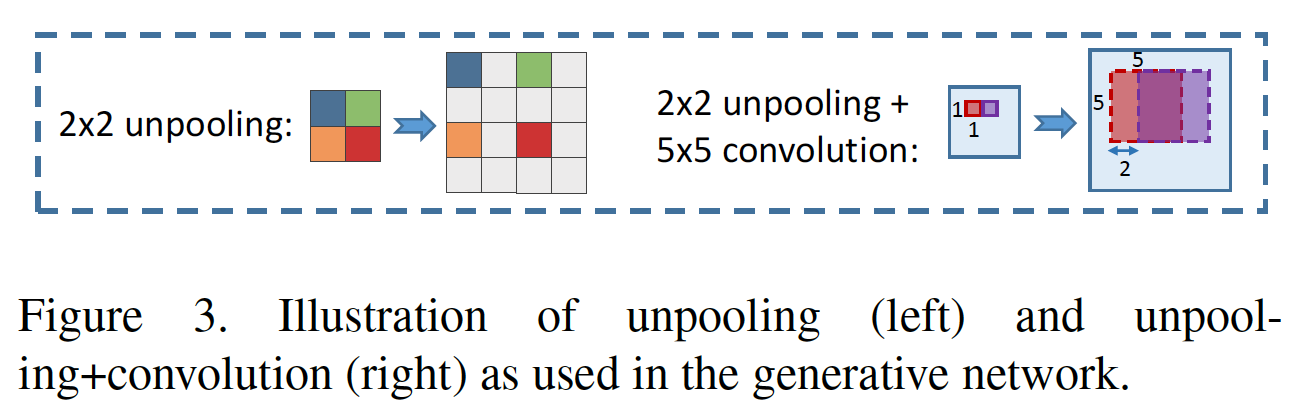
\includegraphics[width=0.9\textwidth]{./figure/dosovitskiy2014fig3.png}
\end{frame}

\begin{frame}[label={sec:orgheadline38}]{20.10.7 Auto-Regressive Networks}
\begin{itemize}
\item Directed probabilistic models with no latent random variables
\item Fully-visible Bayes networks (FVBNs)
\item NADE (Larochelle and Murray, 2011)
\begin{itemize}
\item One type of auto-regressive network
\end{itemize}
\item Reuse of features
\begin{itemize}
\item Statistical advantages (fewer unique parameters)
\item Computational advantages (less computation)
\end{itemize}
\end{itemize}
\end{frame}
\begin{frame}[label={sec:orgheadline39}]{20.10.8 Linear Auto-Regressive Networksv}
\begin{columns}
\begin{column}{0.60\columnwidth}
\begin{itemize}
\item Simplest form of auto-regressive network
\begin{itemize}
\item No hidden units
\item No shared parameters or features
\end{itemize}
\item Examples
\begin{itemize}
\item Logistic auto-regressive network (binary)
\end{itemize}
\item Introduced by Frey (1998)
\item \(O(d^{2})\) parameters (\(d\) variables)
\end{itemize}
\end{column}
\begin{column}{0.40\columnwidth}
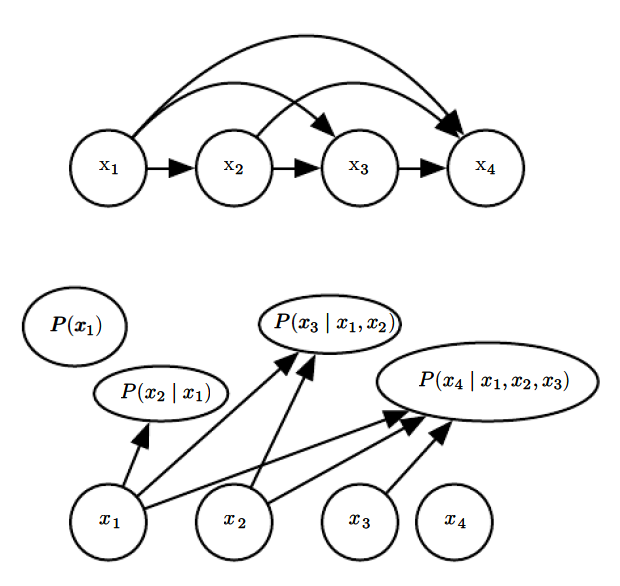
\includegraphics[width=\textwidth]{./figure/dlbook_fig20_8.png}
\end{column}
\end{columns}
\end{frame}

\begin{frame}[label={sec:orgheadline40}]{20.10.9 Neural Auto-Regressive Networks}
\begin{columns}
\begin{column}{0.60\columnwidth}
\begin{itemize}
\item Introduced by Bengio and Bengio (2000a, b)
\item Model capacity can be increased
\item Generalization can be improved by parameter and feature sharing
\item Two advantages of using NN
\begin{enumerate}
\item Can capture nonlinear dependency with limited number of parameters
\item Left-to-right architecture allows one to merge all the NN into one
\end{enumerate}
\end{itemize}
\end{column}

\begin{column}{0.40\columnwidth}
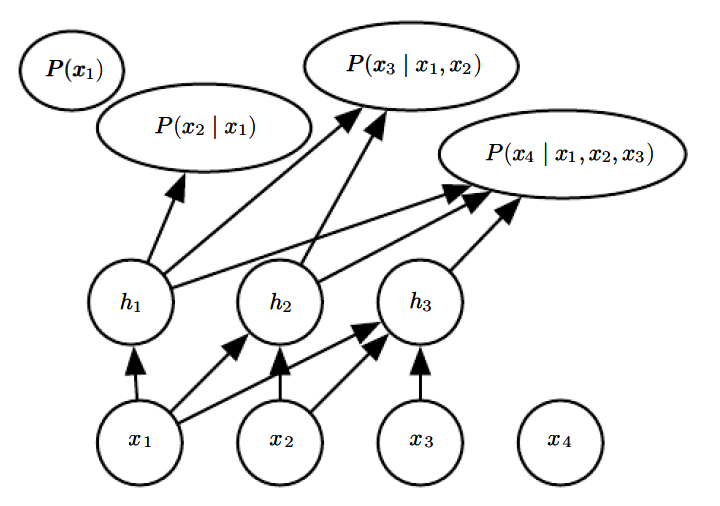
\includegraphics[width=1.1\textwidth]{./figure/dlbook_fig20_9.png}
\end{column}
\end{columns}
\end{frame}

\begin{frame}[label={sec:orgheadline41}]{20.10.10 Neural autoregressive density estimator (NADE)}
\begin{columns}
\begin{column}{0.60\columnwidth}
\begin{itemize}
\item Proposed by Larochelle and Murray (2011)
\item Successful recent form of neural auto-regressive network (NAN)
\item NAN with parameter sharing
\end{itemize}
\begin{align*}
W_{j,k,i}^{'} &= W_{k, i} \tag{20.83} \\
W_{j,k,i}^{'} &= 0 \text{ if } j < i
\end{align*}
\begin{itemize}
\item \(i\) -th input node
\item \(j\) -th hidden node
\item \(k\) -th element of \(j\) -th hidden node
\end{itemize}
\end{column}
\begin{column}{0.40\columnwidth}
\centering
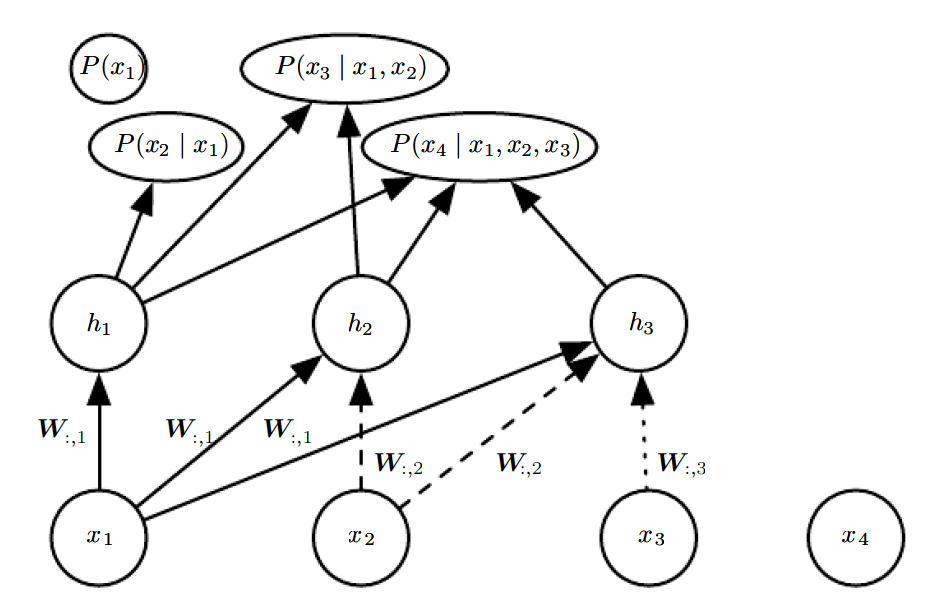
\includegraphics[width=1.1\textwidth]{./figure/dlbook_fig20_10.png}
\end{column}
\end{columns}
\end{frame}

\begin{frame}[label={sec:orgheadline42}]{Variants of NADE}
\begin{itemize}
\item NADE-k (Raiko et al, 2014)
\begin{itemize}
\item k-step mean field recurrent inference
\end{itemize}
\item RNADE (Uria et al., 2013)
\begin{itemize}
\item Processing continuous-valued data using Gaussian mixture
\item Use pseudo-gradient to reduce unstable gradient calculation caused by coupling of \(\mu_{i}\) and \(\sigma_{i}^{2}\)
\end{itemize}
\item Ensemble of NADE models handling reordered inputs \(o\) (Murray and Larochelle, 2014)
\begin{itemize}
\item Better generalization than a fixed-order model
\end{itemize}
\end{itemize}
\begin{align*}
p_{\mathrm{ensemble}}(\bf{x}) = \frac{1}{k} \sum_{i=1}^{k} p(\bf{x} | o^{(i)})
\end{align*}
\begin{itemize}
\item Deep NADE is computationally expensive and not so much gain
\end{itemize}
\end{frame}

\section{20.11 Drawing Samples from Autoencoders}
\label{sec:orgheadline47}
\begin{frame}[label={sec:orgheadline44}]{20.11 Drawing Samples from Autoencoders}
\begin{itemize}
\item Underlying connections between score matching, denoising autoencoders, and contractive autoencoders
\item They are learning data distributions, but how can we sample data?
\item VAE - ancestral sampling
\item CAE 
\begin{itemize}
\item Repeated encoding and decoding with injected noise will induce a random walk along the surface of the manifold (Rifai et al., 2012; Mesnil et al., 2012)
\item Manifold diffusion technique (kind of MC)
\end{itemize}
\item DAE
\begin{itemize}
\item More general MC
\end{itemize}
\end{itemize}
\end{frame}

\begin{frame}[label={sec:orgheadline45}]{20.11.1 Markov Chain Associated with any DAE}
\begin{columns}
\begin{column}{0.50\columnwidth}
\begin{itemize}
\item What noise to inject and where?
\item How to construct such a MC for generalized DAE
\end{itemize}
\end{column}

\begin{column}{0.50\columnwidth}
\centering
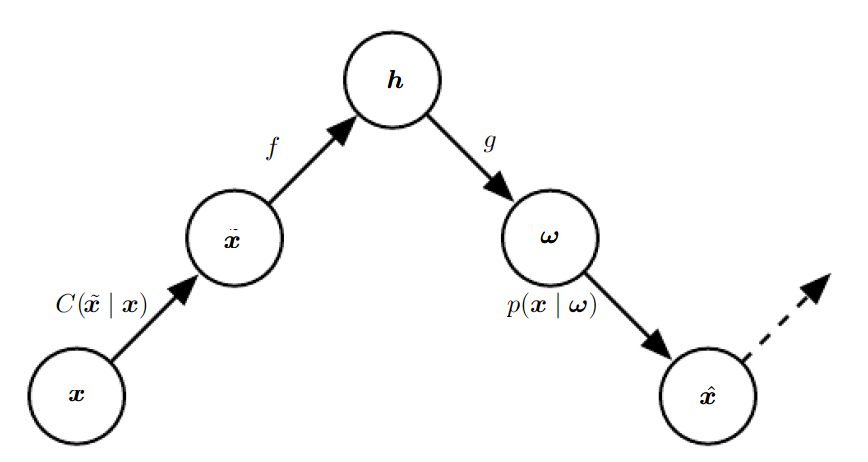
\includegraphics[width=1.1\textwidth]{./figure/dlbook_fig20_11.png}

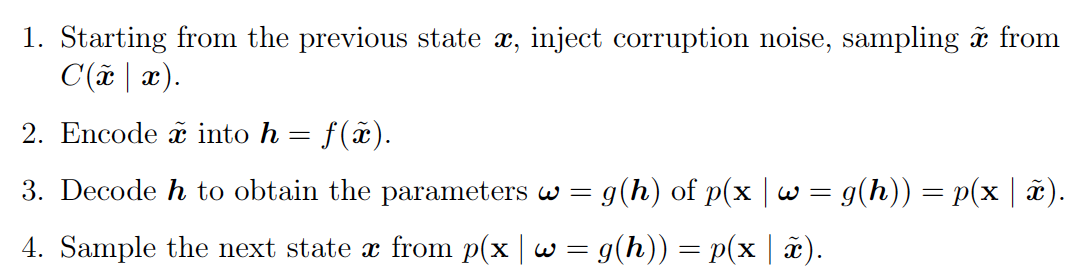
\includegraphics[width=1.1\textwidth]{./figure/dlbook_fig20_11b.png}
\end{column}
\end{columns}
\end{frame}

\begin{frame}[label={sec:orgheadline46}]{20.11.3 Walk-Back Training Procedure}
\begin{itemize}
\item Proposed by Bengio et al. (2013c) to accerelate the convergence rate of generative training of DAE
\item Includes alternative multiple stochastic encode-decode steps
\end{itemize}
\centering
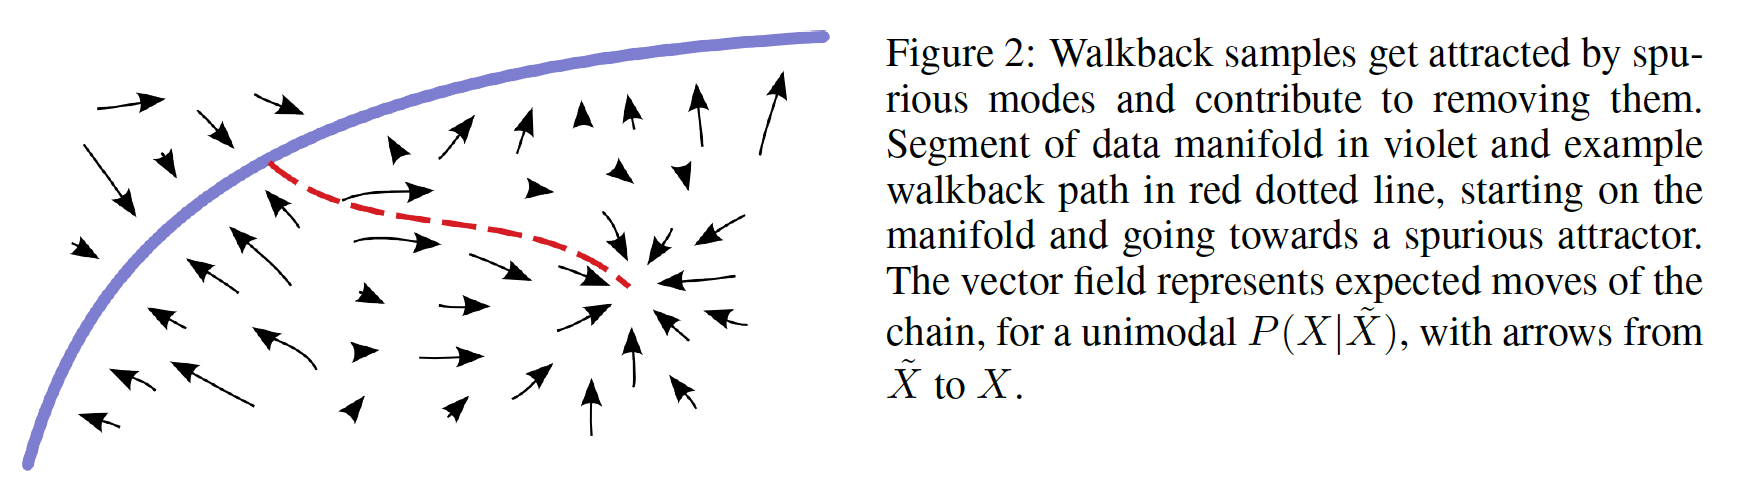
\includegraphics[width=\textwidth]{./figure/bengio2013cfig2.png}
\end{frame}

\section{20.12 Generative Stochastic Networks (GSNs)}
\label{sec:orgheadline50}
\begin{frame}[label={sec:orgheadline48}]{20.12 Generative Stochastic Networks (GSNs) (1/2)}
\begin{itemize}
\item Proposed by Bengio et al. (2014)
\item Generalization of DAE
\begin{itemize}
\item Include latent varialbe \(\bf{h}\) in the generative Markov chain
\end{itemize}
\item Generative process is parameterized by two distributions
\begin{itemize}
\item \(p(\bf{x}^{(k)} | \bf{h}^{(k)})\): reconstruction distribution
\item \(p(\bf{h}^{(k)} | \bf{h}^{(k-1)}, \bf{x}^{(k-1)})\): state transition distribution
\end{itemize}
\end{itemize}

\centering
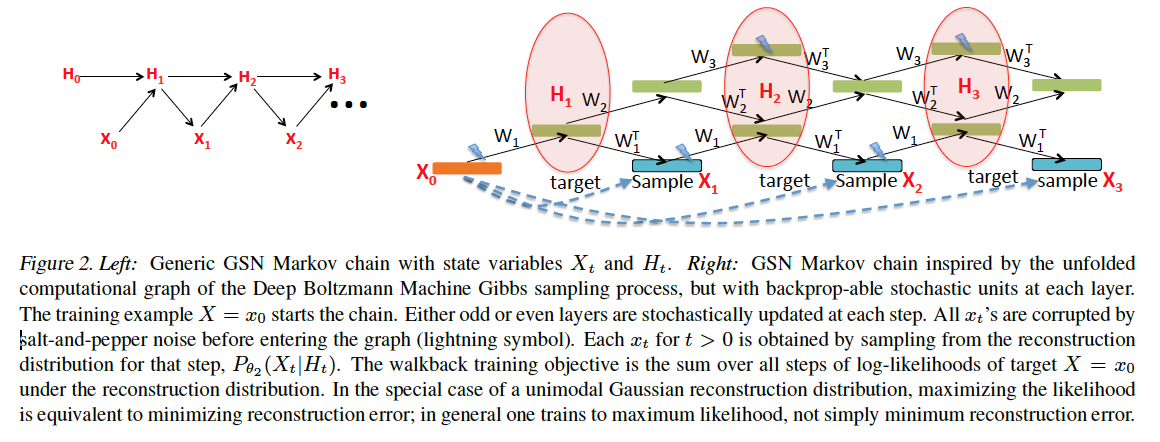
\includegraphics[width=\textwidth]{./figure/bengio2014gsnfig2.png}
\end{frame}


\begin{frame}[label={sec:orgheadline49}]{20.12 Generative Stochastic Networks (GSNs) (2/2)}
\begin{itemize}
\item Properties of GSNs
\begin{itemize}
\item Joint distribution is defined implicitly by MC if it exists
\item Maximize \(\log p(\bf{x}^{(k)} = \bf{x} | \bf{h}^{(k)})\) where \(\bf{x}^{(0)} = \bf{x}\)
\item Walk-back training protocol was used to improve training convergence
\end{itemize}
\item 20.12.1 Discriminant GSNs
\begin{itemize}
\item Possible to model \(p(\bf{y} | \bf{x})\) instead of \(p(\bf{x})\) with GSNs
\end{itemize}
\end{itemize}
\end{frame}

\section{20.13 Other Generation Schemes}
\label{sec:orgheadline52}
\begin{frame}[label={sec:orgheadline51}]{20.13 Other Generation Schemes}
\begin{itemize}
\item So far, MCMC sampling, ancestral sampling, or some mixture of the two
\item Diffusion inversion objective for learning a generative model based on non-equilibrium thermodynamics (Sohl-Dickstein et al., 2015)
\begin{itemize}
\item Structured -> unstructured
\item Running this process backward
\end{itemize}
\item Approximate Bayesian computation (ABC) framework (Rubin et al., 1984)
\begin{itemize}
\item Samples are rejected or modified in order to make the moments of selected functions of the samples match those of the desired distribution.
\item This is not a moment matching because ABC changes the samples themselves
\end{itemize}
\end{itemize}
\end{frame}
\section{20.14 Evaluating Generative Models}
\label{sec:orgheadline56}
\begin{frame}[label={sec:orgheadline53}]{20.14 Evaluating Generative Models (1/2)}
\begin{itemize}
\item Usually we cannot evaluate \(\log p(\bf{x})\) directly
\item Which is better?
\begin{itemize}
\item Stochastic estimate of the log-likelihood for model A
\item Deterministic lower bound on the log-likelihood for model B
\end{itemize}
\item High likelihood estimate \(\log p(\bf{x}) = \log \tilde{p}(\bf{x}) - \log Z\) can be obtained due to
\begin{itemize}
\item Good model, or
\item Bad AIS implimentation (underestimate Z)
\end{itemize}
\end{itemize}
\end{frame}

\begin{frame}[label={sec:orgheadline54}]{20.14 Evaluating Generative Models (2/2)}
\begin{itemize}
\item Changing preprocessing step is unacceptable when comparing different generative models
\begin{itemize}
\item e.g., multiplying the input by 0.1 will artificially increase likelihood by a factor of 10
\item It is essential to compare real-valued MNIST models only to other real-valued models and binary-valued models only to other binary-valued models
\item Use exactly same binalization scheme for all compared models
\end{itemize}
\item Visual inspection can be used but not a reliable measure
\begin{itemize}
\item Poor model can produce good examples by overfitting
\end{itemize}
\item Need to develop some other ways to evaluate generative models
\begin{itemize}
\item You can get extremely high likelihood by asigning arbitrarily low variance to background pixels that never changes
\end{itemize}
\end{itemize}
\end{frame}

\begin{frame}[label={sec:orgheadline55}]{Conclusions}
\begin{itemize}
\item Deep generative models are important building blocks for AI systems
\end{itemize}
\end{frame}
\end{document}
